\section{Branches}\label{sec:branch}
Während der Entwicklung eines Programms ist es meist nützlich mehrere Versionen parallel zu verwalten. Das kann heißen, dass es eine \qq{release} Version und eine \qq{developement} Version gibt. Oder, dass man die letzte funktionierende Variante des Programms erhalten will während man neue Funktionen versucht zu implementieren.

Das parallele nutzen von Entwicklungssträngen ermöglichen Branches in Git.
\subsection{Branch erstellen}
Um einen Branch zu erstellen ruft man \inline{git branch} mit einem Namen für den Branch auf. Dann kann mit \inline{git checkout} zu dem Branch gewechselt werden. Der Log zeigt die Stadien der Branches ebenfalls an.
\begin{lstlisting}
$ git branch section4
$ git checkout section4
$ git log --pretty=format:"%h %s %d"
04965ab add: sentence at end of Commit  (HEAD -> section4, master)
906a721 add: label for future sections 
03a1fee add: Subsection about reverting commits 
bf11cfe add: files to ignore from macOS 
\end{lstlisting}
Hier kann man sehen, dass sowohl master, als auch section4 auf denselben Commit zeigen (\inline{04965ab}). Jeder neue Commit jedoch wird nur von section4 erfasst, nicht von dem master Branch.

\begin{figure}[!ht]
	\centering
	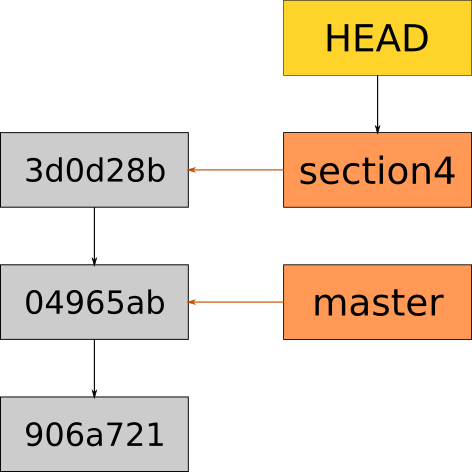
\includegraphics[width=0.4\textwidth]{Bilder/branching.png}
	\caption{Beispielhafter Branch-tree aus diesem Projekt. Graue Kästen stellen einzelne Commits dar, orangene Branches und der gelbe Kasten ist der aktuelle HEAD. Die Pfeile zeigen auf die Verlinkung.}
	\label{fig:branch_1}
\end{figure}
Abb. \ref{fig:branch_1} zeigt den Branch-tree des Gits nach dem ersten Commit in section4. \inline{HEAD} zeigt immer auf den aktuellen Zustand des lokalen Ordners. In diesem Fall auf den Branch section4. Die Branches selber zeigen auf den Commit, den sie gerade darstellen. Um den \inline{HEAD} zu wechseln muss nur \inline{git checkout [BRANCH]} mit dem entsprechenden Branch aufgerufen werden.
\begin{figure}[!ht]
	\centering
	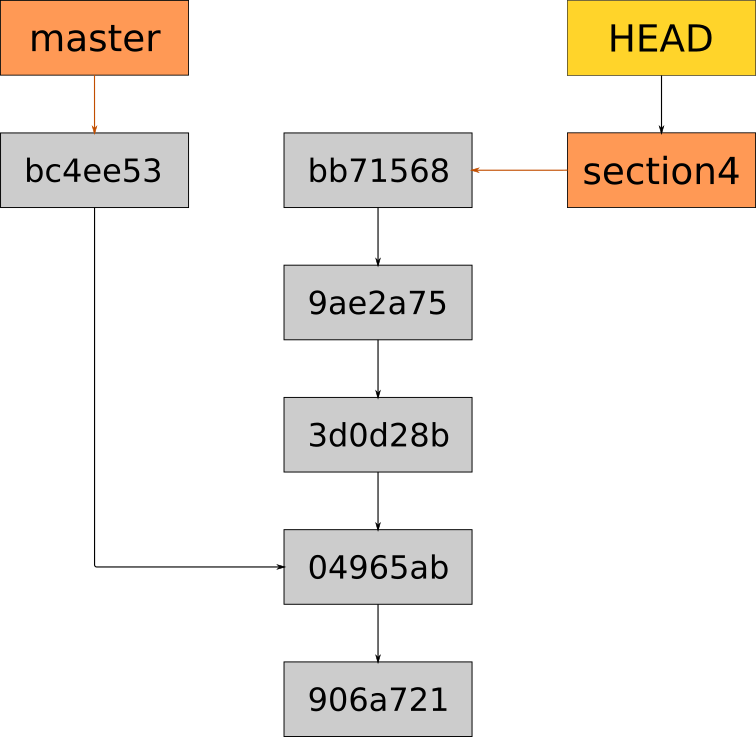
\includegraphics[width=0.4\textwidth]{Bilder/branching_2.png}
	\caption{Branch-tree nachdem mehrere Commits zu den Branches gemacht wurden.}
	\label{fig:branch_2}
\end{figure}

\subsection{Merging}
Das Zusammenführen zweier Branches wird Merging genannt. Dabei ist es das Ziel, alle Änderungen der beiden Branches in einem Branch zu vereinen. Wichtig ist, dass immer der Branch ausgewählt (HEAD zeigt darauf) sein sollte, in dem man die Änderungen vereinen will. Will man also in master die Änderungen von section4 einbinden geht das folgendermaßen:
\begin{lstlisting}
	$ git checkout master
	$ git merge section4
	Merge made by the 'recursive' strategy.
	Bilder/branching.png   | Bin 0 -> 25763 bytes
	Bilder/branching.svg   | 648 ++++++++++++++++++++++++++++++++++++++++++++++++++++++++++++++++++++++++++
	Bilder/branching_2.png | Bin 0 -> 41671 bytes
	branches.tex           |  36 +++++
	main.tex               |   3 +-
	5 files changed, 686 insertions(+), 1 deletion(-)
	create mode 100644 Bilder/branching.png
	create mode 100644 Bilder/branching.svg
	create mode 100644 Bilder/branching_2.png
	create mode 100644 branches.tex
\end{lstlisting}
Merging ist ein einzelner Commit. Dieser Commit zeigt auf die beiden Commits, auf welche die einzelnen Branches vorher gezeigt haben (siehe Abb. \ref{fig:merge}). Nachdem ein Branch gemerged wurde kann er gelöscht werden.
\begin{figure}[!ht]
	\centering
	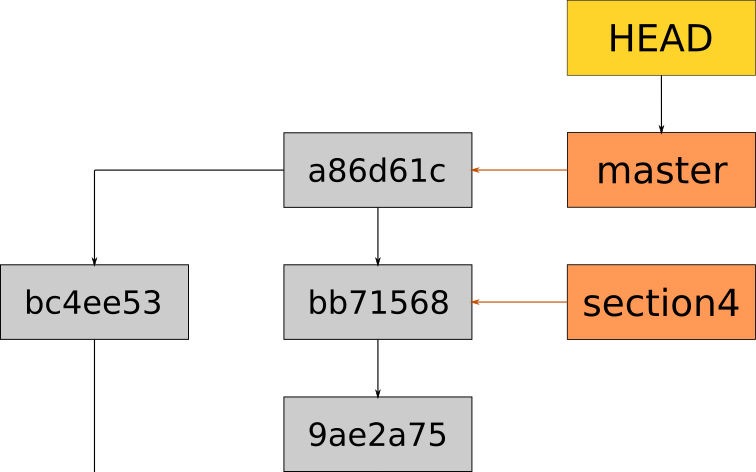
\includegraphics[width=0.6\textwidth]{Bilder/branching_3.png}
	\caption{Branch-tree nach dem Merging. Der Merge wird als eigener Commit oberhalb der beiden child-Commits angezeigt. Der master Branch und HEAD zeigen beide auf den Merge-Commit. Der section4 Branch existiert weiterhin, zeigt jedoch auf den alten Commit.}
	\label{fig:merge}
\end{figure}